\chapter{Implementation Details}
\label{chap:implementation_details}

\subsection{Network Discovery}
\label{sec:network_discovery}
The first thing a device does after booting, is to see which Gateways are in its vicinity and build a routing table out of the information exchanged with their neighbors.
The process is basically the same for all three roles with a few minor differences (see figure \ref{fig:network_discovery}).

\begin{enumerate} [noitemsep]
	\item Once a device has booted, it generates a MAC address, which is nothing more than the hardware's serial number.
	\item A GW\_REQ is broadcasted with the device's MAC address.
		Every Gateway or CS who receives a GW\_REQ, replies with an UPDATE packet. 
		The UPDATE contains the replying Gateway's MAC address and its distance to the CS.
	\item The device will wait all the repies that reach it.
	\item If there were no replies, the process goes back to step 2. 
		Otherwise, each response received is read and evaluated.
	\item The responses with the five best metrics are put in the routing table.
		Gateway metric is reported distance to the CS + weighted RSSI.
		Sensor metric is signal strength.
	\item If the device is a Sensor, it will send a parking status to the best Gateway in its table.
	\item If it is a Gateway, the best metric in the routing table becomes its distance to the CS.
	\item If it is a Gateway or the CS, it will broadcast an UPDATE with its distance to the CS.
	\item Lastly, the device will start its normal operation according to its role.
\end{enumerate}

\begin{figure}
    \centering
    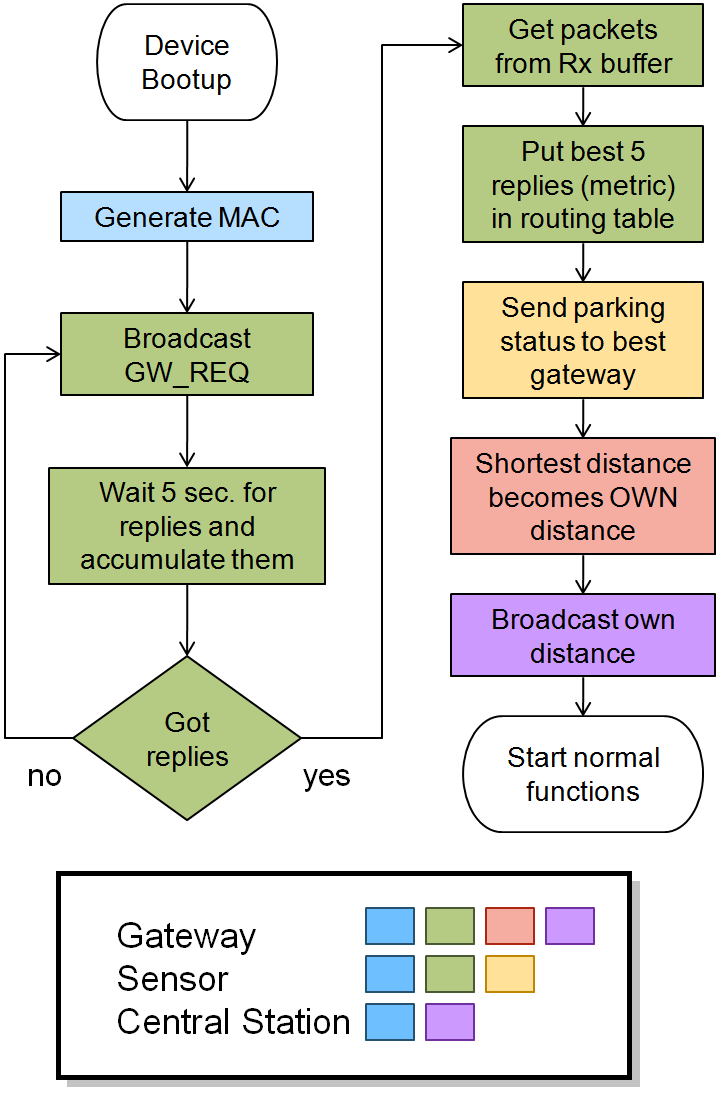
\includegraphics[width=10cm]{images/Flowchart_NetworkDiscovery.png}
	\vspace{-1.5em}
    \caption{Network discovery process for the three roles.}
    \vspace{-1.5em}
    \label{fig:network_discovery}
\end{figure}

\subsection{Parking Status Propagation}
\label{sec:parking_status_propagation}
After a Sensor has built a routing table, it maintains communications with only the Gateway with the best metric.
From this point, the Sensor will spend as little battery as possible.
It can do this this by putting the wireless communications module in sleep mode.
The light sensor (or any other type that best suits the environment) will probe its surroundings periodically to detect any changes.
As soon as the light sensor detects a change, it will send an interruption signal to generate and send the status message.
Then, the process described in figure \ref{fig:sensor} takes place:
\begin{enumerate}[noitemsep]
	\item The Sensor looks in its routing table for the first element (best metric).
	\item If the table is empty, it runs the network discovery process.
		Otherwise, it extracts the MAC address of the first gateway in the table.
	\item The Sensor builds a special packet depending on the current parking status: either OCCUPIED or EMPTY.
		This packet contains the Sensor's MAC address and is destined to address extracted from the table.
	\item The message is sent to its destination and the Sensor waits 300 ms for an acknowledge packet (ACK).
	\item If an ACK is received, the Sensor goes back to sleep mode.
	\item if a NACK is received, the Sensor goes back to step 1 without removing the element from the routing table, but uses the next gateway in the list on step 2.
	\item If the ACK timed out, it tries two more times with the same address.
	\item If there was no response (ACK or NACK), the address to which it tried is removed from the routing table and goes back to step 1.
\end{enumerate}

\begin{figure}
    \centering
    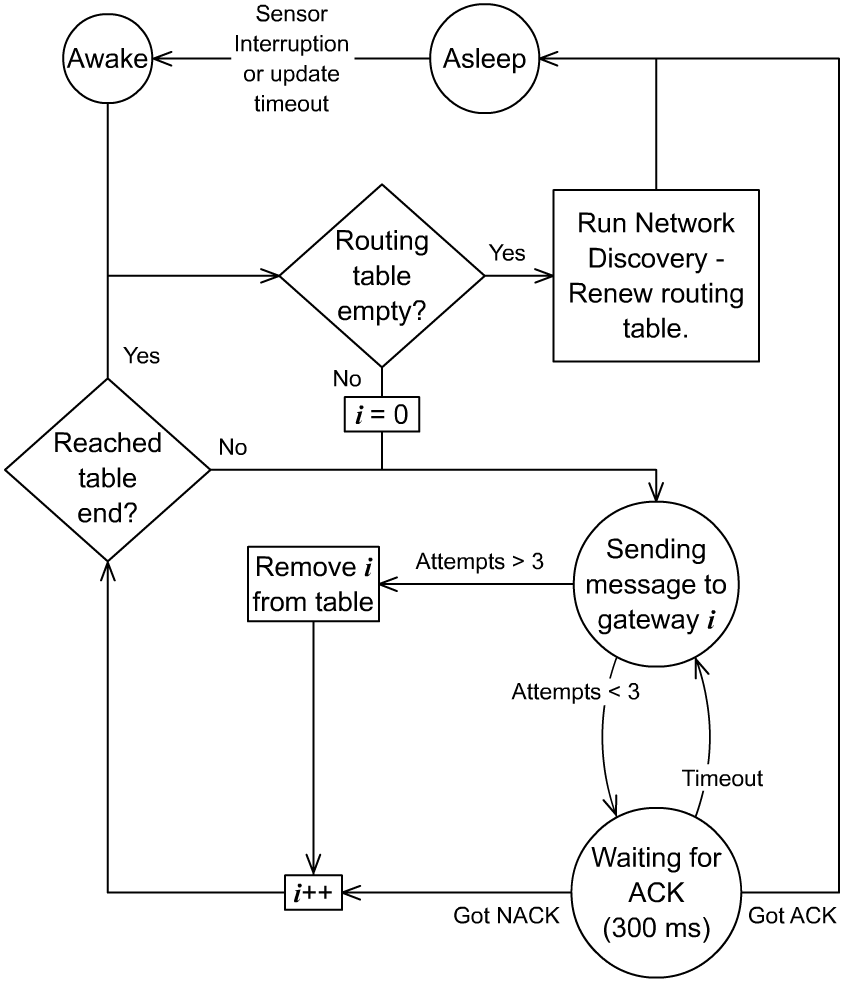
\includegraphics[width=10cm]{images/Flowchart_Mote.png}
	\vspace{-1.5em}
    \caption{Flowchart of the functions of a Sensor.}
    \vspace{-1.5em}
    \label{fig:sensor}
\end{figure}

In the case of a Gateway, the process is very similar. 
The main difference is that a Gateway waits for messages, for its task is to forward them.
It does not go into sleep mode, because it is connected to an "unlimited" source of electricity.
But also, a Gateway sends ACKs if it receives a status message and is currently not busy.
Otherwise, it will send a NACK. The complete process is described in figure \ref{fig:gateway}.

\begin{figure}
    \centering
    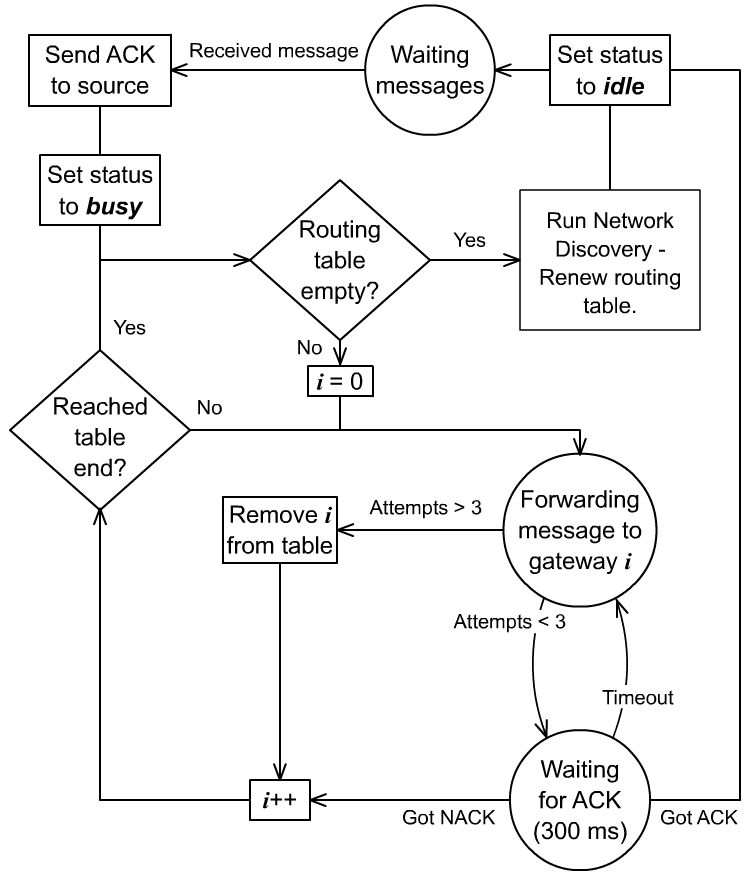
\includegraphics[width=10cm]{images/Flowchart_Gateway.png}
	\vspace{-1.5em}
    \caption{Flowchart of the functions of a Gateway.}
    \vspace{-1.5em}
    \label{fig:gateway}
\end{figure}

\subsection{Packet Format}
\label{sec:packet_format}
In order to provide an agile network convergence, a packet format was devised, which was small, but had the minimum information necessary to meet the system requirements.
Each packet contains four fields (none larger than two bytes): source address, packet ID, command and value.
In the previous sections all five packet types were mentioned in context, but a summary of them can be found in figure \ref{fig:packet}:
\begin{itemize}[noitemsep]
	\item ACK: Used by Gateways to respond to parking status notifications. 
	\item UPDATE: Used by Gateways and the CS to notify neighboring devices of its address and distance to CS.
	\item OCCUPIED: Sent by Sensors to notify a parking space is now occupied.
	\item EMPTY: Sent by Sensors to notify a parking space is now free.
	\item GW\_REQ: Sent by Sensors and Gateways in the network discovery phase to establish communications with neighboring gateways and request the information about distance to the CS.
\end{itemize}

\begin{figure}
    \centering
    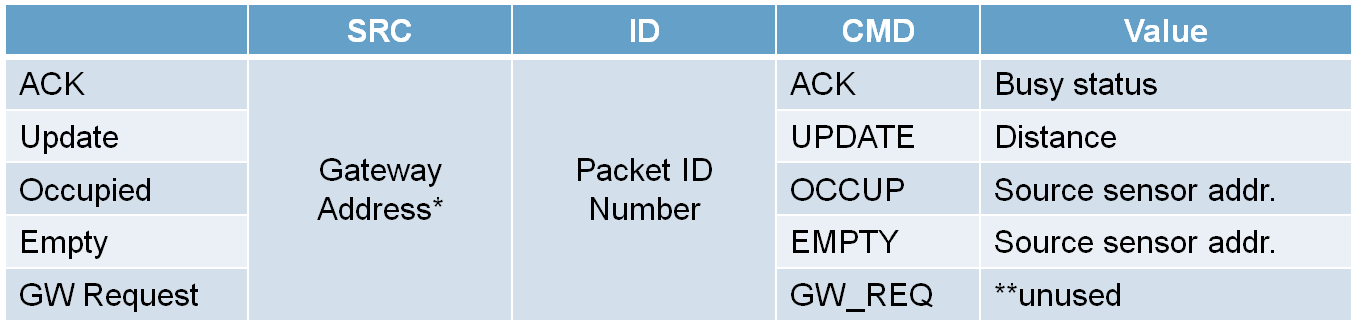
\includegraphics[width=15cm]{images/General_PacketFormat.png}
	\vspace{-1.5em}
    \caption[Packet format]{Packet Format. 
	\(\ast\) In the case of occupied and empty, the SRC field originally contains the Sensor's address.
	\(\ast\ast\) The Packet is fixed length, so the unused value is arbitrarily assigned.}
    \vspace{-1.5em}
    \label{fig:packet}
\end{figure}

\subsection{Graphical User Interface}
\label{sec:gui}
In order to make things lighter for the parking lot operator, a Graphical User Interface (GUI) should provide all the relevant information about the parking and device status as well as some statistics.
For this prototype, we only included the critical information, which is:
\begin{itemize}[noitemsep] 
	\item The number of vacant and occupied parking spaces
	\item A list of Sensors that have connectivity to the CS.
	\item Each Sensor's MAC address.
	\item Number of packets sent by each Sensor
	\item The reported parking status of each Sensor.
	\item The time of the last update of each packet.
\end{itemize}

Additionally a debug output window is included, which shows all messages sent and received by the CS to and from its neighbors (see figure \ref{fig:gui}).

\begin{figure}
    \centering
    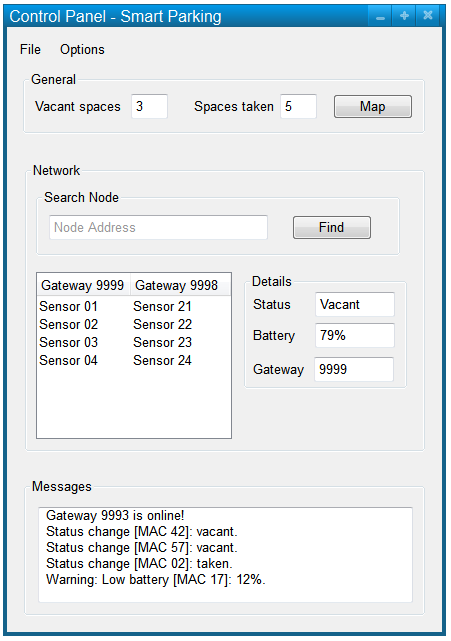
\includegraphics[width=15cm]{images/General_ApplicationGUI.png}
	\vspace{-1.5em}
    \caption{Administrator's GUI}
    \vspace{-1.5em}
    \label{fig:gui}
\end{figure}


